

Finite element methods (FEM's) are capable of modeling nonhomogeneous and anisotropic conductivities within each tissue and therefore will be dependent upon accurate conductivity values for the whole head, but present FEM models are limited by the paucity of conductivity data.

issue boundaries with high conductivity gradients can cause field distortions and lead to localization errors, if the conductivities are not modeled accurately.

%% 
%% The Electrical Conductivity of Human Cerebrospinal Fluid at Body Temperature
%% http://ieeexplore.ieee.org/stamp/stamp.jsp?tp=&arnumber=554770
%% 

\section{Electrical conductivity}

\paragraph{Influence of skull anisotropy for the forward and inverse problem in EEG: simulation studies using FEM on realistic head models~\cite{pmid9704264}}{

{\it is it absolutely necessary to use FEM in order to accurately compute the solution of the EEG inverse problem? Furthermore, under what conditions can BEM provide accurate solutions?  } \\
Considering this fact, the relevant questions are: is it absolutely necessary to use FEM in order to accurately compute the solution of the EEG inverse problem? Furthermore, under what conditions can BEM provide accurate solutions? The most pertinent way to answer these questions is to evaluate the role of anisotropies in the electrical conductivities of brain tissues [Wikswo et al., 1993] and particularly the bone anisotropy, since the presence of the skull greatly influences the scalp potential distribution. Such influence has been evaluated in the forward and inverse dipolar problem by Peters and de Munck [1990] with analytical methods, and by Thevenet [1992] with FEM in a spherical head model. FEM has also been used with a realistic head model [Haueisen et al., 1997], but those authors only studied the influence of conductivity values on the scalp distribution.




For these reasons, the first proposed and still the most commonly used approach to the inverse problem consists in fitting one or a few equivalent current dipolar sources (ECD) to the potential map by nonlinear estimation techniques [Sherg and Buchner, 1993]. Although this model can well describe the focal activities induced by a simple somatosensory study, it is inadequate to represent complex neural networks or distributed activities along cortical surfaces. In order to overcome these difficulties, different tomographic reconstruction techniques have been proposed which estimate a distribution of current vectors on a regular surface grid [Hamalainen and Ilmoniemi, 1984] or a volume grid [Pascual-Marqui et al., 1994] or cortical surface deduced from MRI images [Dale and Sereno, 1993]. The {\it distributed sources} inverse problem consists in solving a set of linear equations, since the locations of the currents are imposed, but this system is undetermined since there are many more unknowns than the number of data. Then constraints must be introduced in order to limit the set of admissible solutions in a so-called regularization scheme. The most commonly used are minimum norm estimates (Hamalainen and Ilmoniemi, 1994; Wang et al., 1992] or quadratic regularizations that generate smooth distributions, not corresponding to realistic physiological solutions.

Different head models have been used, and the complexity of the corresponding potential calculations increases with the accuracy of the head description. The simplest and the most commonly used is the three or four concentric sphere model with homogeneous conductivity values which represent the skin, the skull, the Cerebrospinal Fluid (CSF), and the brain tissues. In this case, analytical expressions have been derived to calculate the scalp potentials [De Munck, 1988]. Spherical models may take into account anisotropy of the medium by assigning constant radial and tangential conductivities to the skull shell, but they give a poor approximation of head shape. In order to take into account realistic head geometry, Hamalainen and Sarvas [1989] used the boundary element method (BEM), which is adequate for piecewise homogeneous isotropic media. However, BEM cannot be applied when some inhomogeneities are present (such as skull holes) or when the medium has an anisotropic conductivity. Indeed, anisotropy influences the scalp potential distributions [Peters and de Munck, 1990]. In such a case, the finite element method (FEM) allows one to consider accurate inhomogeneous realistic models, since it computes the Maxwell equations very locally. Different authors have developed FEM methods [Yan et al., 1991; Bertrand et al., 1991; Haueisen et al., 1995; Buchner et al., 1997; Awada et al., 1997]. FEM is difficult to implement since it requires volume meshes of the different head tissues, which are more complex to derive than the surface meshes used by BEM. For this reason, FEM is less commonly used than BEM, even though it is more accurate.


More precisely, for this study, FEM is implemented and validated in the spherical case in comparison with analytical results, and the optimum characteristics of the numerical methods are derived. Then the influence of skull anisotropy on scalp potential is evaluated by comparing the distributions obtained with and without anisotropy both in a spherical and in a realistic head model. To derive the influence of the skull isotropic conductivity approximation in the inverse problem, the gain matrix is computed with an isotropic forward model and a distributed source model is reconstructed with this matrix from data simulated with FEM and an anisotropic skull model. As for the forward problem, spherical and realistic head models are considered and the reconstructions are computed with the different regularization methods mentioned above. We have checked that each inverse method succeeds at recovering accurately the source distribution when the gain matrix is computed with the right anisotropic model.

{\bf Methods FEM description ...}


}

\paragraph{A finite difference method with reciprocity used to incorporate anisotropy in electroencephalogram dipole source localization~\cite{pmid16077227}}{
EEG dipole source localization consists of two subproblems, i.e., the forward and the inverse problem. The forward problem calculates the electrode potentials in a head model, given the source(s) (usually a current dipole). On the other hand, the inverse problem is solved by finding the dipole which best represents the given potentials at the scalp electrodes. 

The skull consists of three layers: a spongiform layer between two hard layers. The conductivity tangentially to the skull surface is 10~times larger than the radial conductivity. White matter consists of axons, grouped in bundles. The conductivity along the nerve bundle is 9 times larger than perpendicular to the nerve bundle.
}

\section{Diffusion tensor imaging (DTI)}

\paragraph{Diffusion Tensor Imaging of the Brain~\cite{citeulike:1695483}}{
Diffusion tensor imaging (DTI)\index{Diffusion tensor imaging} is used to map and characterize the three-dimensional diffusion of water. The diffusion tensor describes the magnitude, the degree of anisotropy, and the orientation of diffusion anisotropy~\cite{citeulike:1695483}.\\
Diffusion is a random transport phenomenon, which describes the transfer of water molecules. In three dimensions, the Einstein diffusion equation:

$$
D = \frac{<\Delta r^{2}>}{2n \Delta t}
$$

states that the diffusion coefficient, $D$ (in mm$^{2}$/s), is proportional to the mean squared-displacement, $<\Delta r^{2}>$ divided by the number of dimensions, $n$, and the diffusion time, $\Delta t$.\\
In the absence of boundaries, the molecular water displacement is described by a Gaussian probability density

$$
P \{\Delta r, \Delta t\} = \frac{1}{\sqrt{(2 \pi D \Delta t)^{3}}} \exp \left \lbrace - \frac{\Delta r^{2}}{4 D \Delta t} \right \rbrace
$$

The spread in this distribution increases with the diffusion time, $\Delta t$.\\

Cellular membranes hinder the diffusion of water, causing water to take more tortuous paths, thereby decreasing the mean squared displacement. The application of the diffusion tensor to describe anisotropic diffusion behavior was introduced by Basser et al.{\bf 1,2} In this elegant model, diffusion is described by a multivariate normal distribution


$$
P \{\Delta \vec{r}, \Delta t\} = \frac{1}{\sqrt{(4 \pi \Delta t)^{3} |\Bar{\bar{D}}|}} \exp \left \lbrace - \frac{(\Delta \vec{r})^{T} \Bar{\bar{D}}^{-1} \Delta \vec{r}}{4 \Delta t} \right \rbrace
$$

where the diffusion tensor $\Bar{\bar{D}}$ is a $3 \times 3$ covariance matrix

$$
\Bar{\bar{D}} = 
\left(
\begin{array}{ccc}
D_{xx} & D_{xy} & D_{xz} \\
D_{yx} & D_{yy} & D_{yz} \\
D_{zx} & D_{zy} & D_{zz} \\
\end{array}
\right)
$$

which describes the covariance of diffusion displacements in 3D normalized by the diffusion time. The diagonal elements ($D_{ii} > 0$) are the diffusion variances along the $x$, $y$ and $z$ axes, and the off-diagonal elements are the covariance terms and are symmetric about the diagonal ($D_{ij} = D_{ji}$). Diagonalization of the diffusion tensor yields the eigenvalues ($l_{1}$, $l_{2}$, $l_{3}$) and corresponding eigenvectors ($\hat{e}_{1}$, $\hat{e}_{2}$, $\hat{e}_{3}$) of the diffusion tensor, which describe the directions and apparent diffusivities along the axes of principle diffusion. The diffusion tensor may be visualized using an ellipsoid with the eigenvectors defining the directions of the principle axes and the ellipsoidal radii defined by the eigenvalues (see figure~\ref{nihms26625f2}. Diffusion is considered isotropic when the eigenvalues are nearly equal (e.g., $l_{1} \sim l_{2} \sim l_{3}$). Conversely, the diffusion tensor is anisotropic when the eigenvalues are significantly different in magnitude (e.g., $l_{1} > l_{2} > l_{3}$).\\
Water diffusion is usually more anisotropic in white matter regions, and isotropic in both gray matter and cerebrospinal fluid. The major diffusion eigenvector ($\hat{e}_{1}$ -- direction of greatest diffusivity) is assumed to be parallel to the tract orientation in regions of homogenous white matter. This directional relationship is the basis for estimating the trajectories of white matter pathways with tractography algorithms.\\

\begin{figure}[htbp]
   \begin{center}
%% \ifx \PDF \undefined
%%       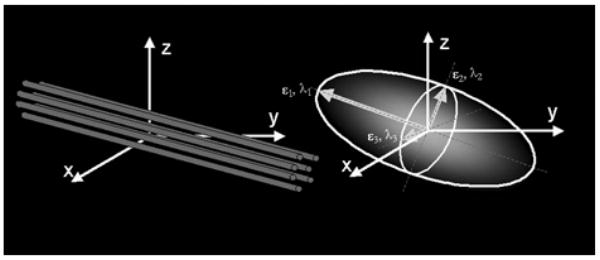
\includegraphics[width=9cm,height=5cm]{images/nihms26625f2.jpg}\hfill
%% \else
      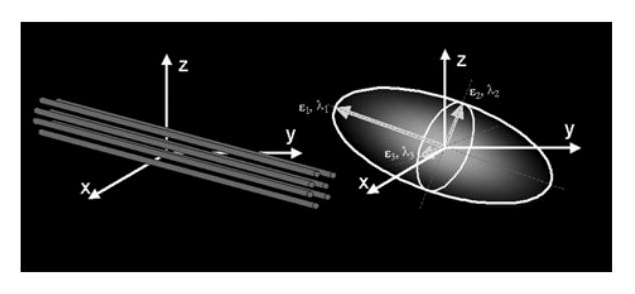
\includegraphics[width=9cm,height=5cm]{images/nihms26625f2.eps}\hfill

%% \fi
   \end{center}
   \caption{\label{nihms26625f2} Diffusion displacement distributions for the diffusion tensor. The diffusion is highly anisotropic in fibrous tissues such as white matter and the direction of greatest diffusivity is generally assumed to be parallel to the local direction of white matter~\cite{citeulike:1695483}.}
\end{figure}

The display, meaningful measurement, and interpretation of 3D image data with a $3 \times 3$ diffusion matrix at each voxel is a challenging or impossible task without simplification of the data. Consequently, it is desirable to distill the image information into simpler scalar maps. The two most common measures are the trace and anisotropy of the diffusion tensor. The trace of the tensor, or sum of the diagonal elements of $\Bar{\bar{D}}$, is a measure of the magnitude of diffusion and is rotationally invariant. The MD (often called the apparent diffusion coefficient or ADC) is used in many published studies and is simply the trace divided by three (MD = Tr/3), which is equivalent to the average of the eigenvalues. Many measures of anisotropy have been described, most of which are rotationally invariant.}

\paragraph{Diffusion tensor imaging: Concepts and applications~\cite{lebihan2001}}{
Water molecules move in the brain on average over distances around 10~$\mu$m, bouncing, crossing, or interacting with many tissue components such as cell membranes, fibers, or macromolecules.

The overall effect observed in a diffusion MRI image voxel of several mm$^{3}$ reflects, on a statistical basis, the displacement distribution of the water molecules present within this voxel. The observation of this displacement distribution may thus provide unique clues to the structure and geometric organization of tissues.

This anisotropy may result from a peculiar physical arrangement of the medium (such as in liquid crystals) or the presence of obstacles that limit molecular movement in some directions. As diffusion is encoded in the MRI signal by using magnetic field gradient pulses (8), only molecular displacements that occur along the direction of the gradient are visible. The effect of diffusion anisotropy can then easily be detected by observing variations in the diffusion measurements when the direction of the gradient pulses is changed. This is a unique, powerful feature not found with usual MRI parameters, such as T1 or T2.

Diffusion anisotropy in white matter originates from its specific organization in bundles of more or less myelinated axonal fibers running in parallel, although the exact mechanism is still not completely understood: diffusion in the direction of the fibers is faster than in the perpendicular direction. It quickly appeared that this feature could be exploited to map out the orientation in space of the white matter tracks in the brain using a color scale, assuming that the direction of the fastest diffusion would indicate the overall orientation of the fibers.

To determine the diffusion tensor fully, one must first collect diffusion-weighted images along several gradient directions, using diffusion-sensitized MRI pulse sequences such as echoplanar imaging (EPI). As the diffusion tensor is symmetric, measurements along only six directions are mandatory (instead of nine).}

\section{Conductivity tensor}

\paragraph{Conductivity tensor mapping of the human brain using diffusion tensor MRI~\cite{Tuch25092001}}{
Here, using an effective medium approach, we show how the electrical conductivity tensor of tissue can be quantitatively inferred from the water self-diffusion tensor as measured by diffusion tensor magnetic resonance imaging.

Excitable tissues such as nerve and muscle mediate communication through electrical currents. These endogenous currents are capable of generating electromagnetic fields sufficiently large to be measured outside of the body by using, for example, electro/magnetoencephalography (EEG/MEG) in the case of the brain or electro/magnetocardiography (ECG/MCG) for the heart.

Efforts to develop an imaging modality to quantitatively measure the electrical conductivity of tissue noninvasively have largely been thwarted by anatomical and biophysical barriers: the organ of interest can be shielded by highly resistive barriers such as the bony tissue of the skull, and the tissue can exhibit significant reactance, anisotropy, and microstructural heterogeneity.

DTI employs an pulsed-gradient spin echo to measure the self-diffusion tensor of water in the tissue (13). The hypothesized relationship between electrical conductivity and water self-diffusion in tissue is prompted by the observation that, although there is no fundamental relationship between the two transport modes in free solution, in a structured medium such as tissue the two processes are related through mutual respect for the boundary conditions imposed by the tissue geometry.

 To derive the cross-property relation between the conductivity and diffusion tensors in brain tissue, the approach we adopt here is to estimate the statistical moments of the microstructure from the observed diffusion tensor, and then derive the conductivity tensor from the estimated moments. We assume in the following that the cell membrane is freely permeable to water and impermeable to charge-carriers on the experimental time scale ($\sim$~50~ms). Following Sen and Torquato.
 
The two-phase model consisting of an inclusion phase embedded in a host phase is particularly amenable to describing biological tissues because the extracellular space can be taken as the host phase and the intracellular space as the inclusion phase.
 
Following Sen and Torquato (22), the effective transport tensor $\Bar{\bar{\Lambda}}$, denoting either the effective electrical conductivity tensor $\Bar{\bar{\sigma}}$ or the diffusion tensor $\Bar{\bar{D}}$, for a two-phase anisotropic medium of arbitrary topology is given by
%% 
%% eq1
%% 
where $\varphi_{i}$ is the inclusion (intracellular) volume fraction, $\Bar{\bar{U}}$ is the identity tensor, and $\lambda_{i}$ and $\lambda_{e}$ are, respectively, the inclusion (intracellular) and host medium (extracellular) transport coefficients; for example, in the case of diffusion $d_{i}$ is the intracellular diffusion coefficient and $d_{e}$ is the extracellular diffusion coefficient. Similarly, $\sigma_{i}$ is the intracellular conductivity value and $\sigma_{e}$ is the extracellular conductivity. The dimensionless contrast factors $\beta$ and $\Bar{\bar{B}}$ are defined as

%% 
%% eq2 et eq3
%% 

The rank-2 tensors $A_{n}^{(i)}$ contain the microstructure information and are defined as integrals over the $n$-point probability functions $S_{n}^{i}$, which give the probability of finding $n$ points within the inclusion (intracellular) phase. Exact expressions for $A_{n}^{(i)}$ are available in ref. 22.
By setting $A_{1}^{(i)} = - \phi_{i} \Bar{\bar{U}}$, the first term on the right-hand side of Eq. 1 can be embedded in the sum to give 

%%
%% eq 4
%% 

where we have defined $\beta_{\lambda} = \beta(\lambda_{i}, \lambda_{e})$ \dots

{\bf Results} \\
The full fractional linear relationship (Eq. 11) was fit to the conductivity and diffusion data, as was a linear relationship of the form $\sigma_{nu} = k(d_{\nu} - d_{\varepsilon})$ for comparison. The linear fit yielded $k = 0.844 \pm 0.0545$~S.s/mm$^{3}$ and $d_{\varepsilon} = 0.124 \pm 0.0540~\mu$m$^{2}$/ms $r^{2} = 0.945$.
}
